\usepackage{ifxetex}
\ifxetex
    \usepackage{fontspec}
    \usepackage{xunicode}
    \usepackage{xltxtra}
    \usepackage{xecyr}
    \usepackage{polyglossia}

    \setmainlanguage{english}
    \setotherlanguages{russian}
\else
    \usepackage[T1]{fontenc}
    \usepackage[utf8]{inputenc}
    \usepackage{lmodern}
\fi

%% USAGE: 
% \usepackage[logo=sklogo]{beamerskoltech} 
%   if you have a stand-alone image file for Sk logo 
% or
% \usepackage[logo]{beamerskoltech} 
%   if you has no logo-file, but want LaTeX to generate it. 
%   In this case you probably will need to use `--enable-write18 -interaction=nonstopmode` arguments running the latex command.
%   in papeeria and overleaf all works fine
% or 
% \usepackage{beamerskoltech}
%   In case you don't want logo at all 
%
% provided commands:
% color `skoltechgreen` -- the dark-green color for structure elements 
% command `\logoname` -- the name of logo file if exist 
% command `{\csk <text>}` -- the shortcut from `\color{skoltechgreen}`
% command `skfootnote{text}` -- put some text for current slide
% `\renewcommand{\skbeforetitle}{\vspace{-3ex}}` is useful in case you use `aspectratio=169`. Also for this aspectratio it is useful to make `\setlength{\skfootnotelen}{12cm}`
%%%%%%%%%%%%%%%%
\usepackage[logo=sklogo]{beamerskoltech} 
\usefonttheme[onlymath]{serif}

\usepackage{amsmath}
\usepackage{amssymb}
\usepackage{amsfonts}

\usepackage{hyperref}

\usepackage[natbib=true]{biblatex}
\usepackage{bibentry}
\usepackage{doi}
\addbibresource{references.bib}

\usepackage{tikz}
\usepackage{pgfplots}
\usetikzlibrary{calc}

\title{Geometric Deep Learning}
\subtitle{for Inverse Graphics}
\author{Serge Kozlukov}
\institute{Skoltech}
\date{June 5, 2020}

\begin{document}

\frame{\titlepage}

\note{
    Salut! My name's Serge,
    I'm supervised by Dmitry Ulyanov
    and Vladimir Spokoiny,
    and the subject of my thesis is:
    ``Geometric Deep Learning for Inverse Graphics''.
}

\begin{frame}\frametitle{Background}
    \begin{itemize}
            \item Hyperbolic DL
            \item Equivariant CNNs
            \item Graph-convolutional NNs
    \end{itemize}
\end{frame}

\note{
There will be three manifestations of ``geometric methods''
that we shall be concerned with in this talk, namely:
\begin{itemize}
    \item Hyperbolic Deep Learning, concerned with the notion of \emph{curvature}
    \item Equivariant convolutional networks, which, as functions, try to
        preserve the symmetric structure of their input and output
        spaces
    \item Finally, Graph-convolutional networks, that operate directly on
        irregular data, like graphs, texts, or pointclouds.
\end{itemize}
}

\begin{frame}{Background: Hyperbolic DL}
    \framesubtitle{Curvature bounds}

    \begin{itemize}
        \item \( M \) a metric space,
        \item \( p, q, r \in M \),
        \item \( \bar{p}, \bar{q}, \bar{r} \in \mathbb{R}^2 \) -- a comparison triangle,
        \item \( \gamma_t \in M \) on the geodesic between \( q, r \),
        \item \( |\bar{p}\bar{\gamma}_t| > |p\gamma_t| \):
    \end{itemize}

    \begin{figure}\centering
        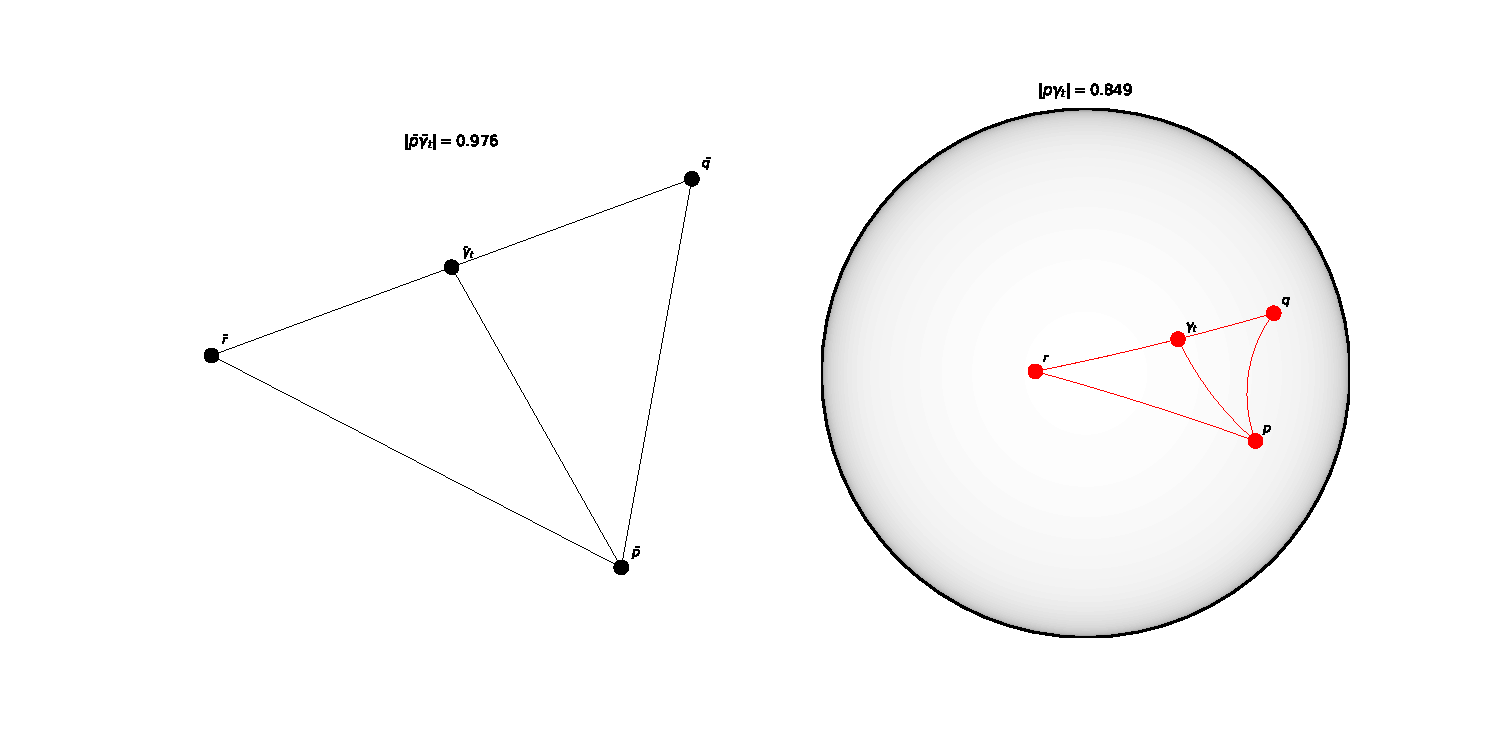
\includegraphics[width=.85\linewidth]{art/triangle-comparison.pdf}
    \end{figure}
\end{frame}

\note[itemize]{
    \item First, I'd like to talk about the hyperbolic deep learning.
        For this discussion we need to clarify what a hyperbolic space is
        or, more generally, what are spaces of \emph{negative curvature}.
    \item By that we understand a metric space whose distance function enjoys
        a certain inequality.
    \item For instance, consider a triangle formed by points \(p, q, \) and \( r \)
        in our space, connected by shortest paths.
    \item The distance from point \( p \) to a point \( \gamma_t \) on the
        opposite side in a negatively curved space will be strictly less than
        the same distance in a similar triangle in Euclidean plane.
}

\begin{frame}{Background: Hyperbolic DL}
    \framesubtitle{Metric graphs}

    \begin{columns}
        \begin{column}{.45\linewidth}
            \begin{figure}\centering
                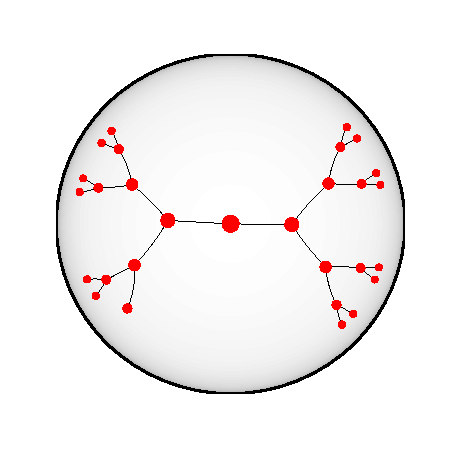
\includegraphics[width=.95\linewidth]{art/h-binary-tree.pdf}
                \caption{Binary tree: \( 2^{n+1}-1 \)
                points on first \( n \) levels}
            \end{figure}
        \end{column}
        \begin{column}{.45\linewidth}
            \begin{figure}\centering
                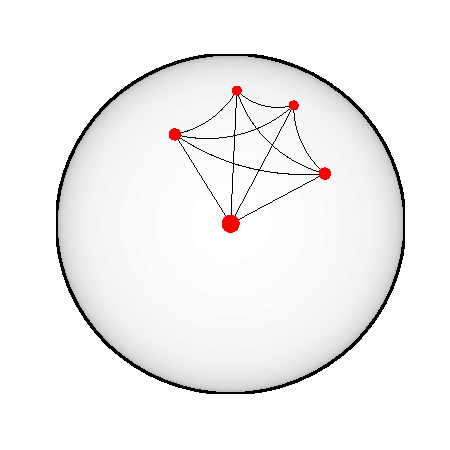
\includegraphics[width=.95\linewidth]{art/h-clique.pdf}
                \caption{Clique: \( n \) mutual nearest neighbours}
            \end{figure}
        \end{column}
    \end{columns}
\end{frame}

\note[itemize]{
    \item A trivial yet conceptually useful example of a negatively curved space
        can be constructed using graphs.
    \item A graph, naturally, is a metric space: its points are the nodes of
        the graph, and distances are measured in the number of edges between
        points.
    \item A full binary tree is a discrete example of a Hyperbolic space.
        One of its characteristic features is the exponential volume growth.
        The ball of radius \( n \),
        centered at the root of the tree contains all the nodes on
        its first \( n \) levels, which is the order of \( 2^{n} \) points.
}
\note[itemize]{
    \item Another unique configuration we could realize with graphs, is the space
        where any number of points are simultaneously nearest neighbours
        of each other.
    \item At the same time, in the Euclidean plane one could only allocate three.
    \item This has a number of implications when we try to define a notion of
        similarity of objects in terms of distance between their embeddings.
    \item This suggests to learn representations of data in a Hyperbolic space,
        and has inspired a series of works applying this idea, for example,
        in Language Modeling.
}

\begin{frame}{Background: Hyperbolic DL}
    \framesubtitle{Curvature in image classifiers}

    \begin{columns}
        \begin{column}{.5\linewidth}
            \begin{itemize}
                    \item ``Hyperbolic Image Embeddings''
                    \item Distance between embeddings is NPC
            \end{itemize}
        \end{column}
        \begin{column}{.5\linewidth}
            \begin{figure}\centering
                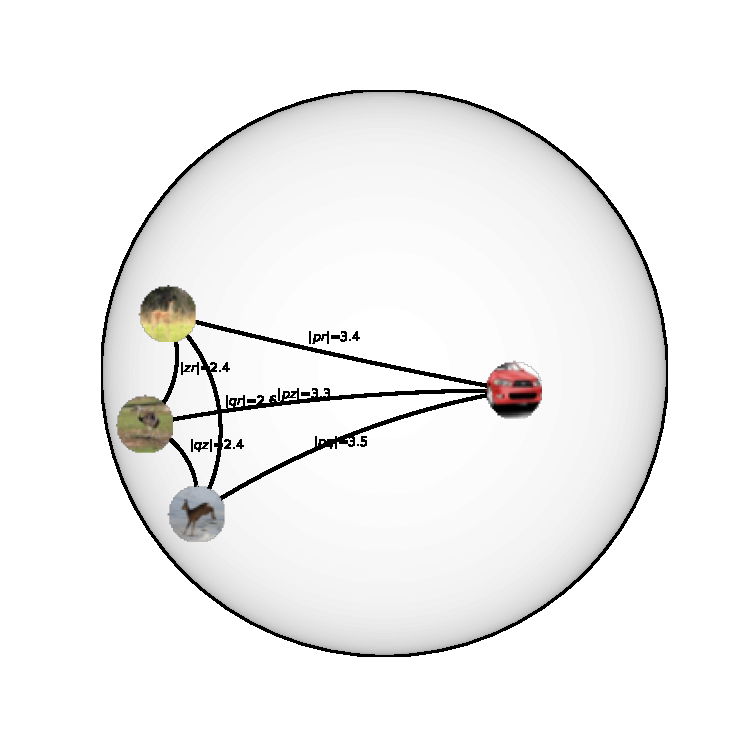
\includegraphics[width=.95\linewidth]{art/quadruple-8.pdf}
            \end{figure}
        \end{column}
    \end{columns}
\end{frame}

\note[itemize]{
    \item The intuition is that Hyperbolic spaces are good at capturing
        hierarchical relationships, but!
    \item It has also been hypothesized that hyperbolic embeddings could be
        of use in problems that exhibit not explicit hierarchies,
        but rather ``latent'' ones.
    \item The ``Hyperbolic Image Embeddings'' paper demonstrates that image
        classifiers are, in a way, trying to learn a negatively curved
        distance function. They further improve the baselines by explicitly
        introducing hyperbolic representations into the model.
}

\begin{frame}{Background: Hyperbolic DL}
    \framesubtitle{Convolutions for ``hyperbolic arrays''}\centering

    \begin{figure}\centering
        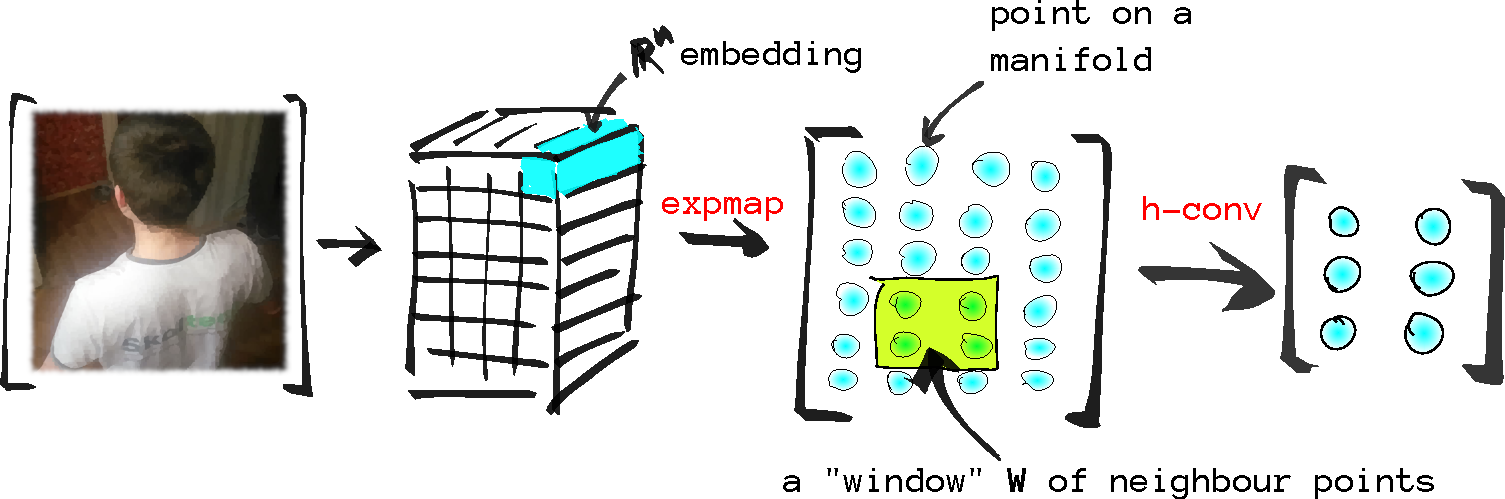
\includegraphics[width=\linewidth]{art/image-convolutions-2019.pdf}
    \end{figure}

        \[ x' = \exp_0\left(
            \operatorname{Conv2D}\left(
                \log_0(y)
                \right)\right) \]

        Kochurov, Karimov, Taktasheva, Mazur, Kozlukov
\end{frame}

\note[itemize]{
    \item This sets the quest to construct composable neural layers that
        operate on hyperbolic embeddings directly.
    \item In an earlier collaborative project we've evaluated the following
        approach:
    \item We consider the image classification problem.
    \item After we've fed an image into a vanilla convolutional network, we
        obtain an \( 3 \)-dimensional array with two spatial indices and one
        feature index.
    \item We could interpret it as a \( 2 \)-dimensional array
        of points in a curved space...
    \item ...which we could scan with a sliding window,
        and each time apply a ``magic'' to the points in the window,
        to produce a single output point.
}
\note[itemize]{
    \item The ``magic'' assumes conversion of points into vectors, the
        application of some blackbox operation, and conversion back into
        points. More on that later.
    \item The model has left a number of questions open
    \item For instance, it suffered heavily from overfitting
}

\begin{frame}{Background}
    \framesubtitle{Equivariance}

    \[
        f \mathbin{*} g = x \mapsto \int_G f(g e) h(g^{-1} x) \operatorname{d}g
    \]

    \begin{itemize}
        \item Classic: \( (G, e, +, -), \) \( G=\mathbb{R}^n, \) \( e=0, \)
            \( g^{-1}x = x - g. \)
        \item \( * \) commutes with translations:
            \( g\circ (f \mathbin{*} h)
            = (g \circ f) \mathbin{*} h
            = f \mathbin{*} (g^{-1} \circ h). \)
        \item S2CNN (Cohen, Welling): \( \operatorname{dom}f = S^2, \)
            \( G = \operatorname{SO}(3) \).
    \end{itemize}
\end{frame}

\note[itemize]{
    \item Another branch of geometric methods is concerned with equivariance.
    \item The defining property of convolutions is that they are the only
        linear operators that commute with translations: it doesn't matter
        if you translate the image before or after convolution.
    \item It is understood that the tremendous success of classic convolutional
        networks is due to their pattern-matching behaviour, which is possible
        precisely because of that property.
    \item However, some data may exhibit symmetries other than translational.
    \item For instance, Cohen et Welling consider problems with spherical
        inputs (think of a heatmap over the surface of the earth).
    }
\note[itemize]{
    \item It turns out that people have been studying convolutions and the rest
        of Harmonic Analysis in the context of arbitrary groups and semirings.
    \item The key insight to generalization is that the integral in the
        convolution formula isn't over the \emph{domain} of the function \( f\),
        but over the group \( G \) of transformations acting on the domain.
}

\begin{frame}{Background: Deep Learning on Graphs}
    \framesubtitle{Message passing and EdgeConv}

    \begin{columns}
        \begin{column}{.45\linewidth}
            ``Message passing''
            \begin{itemize}
                    \item Edge list representation
                    \item \( x \) -- source
                    \item \( y \) -- destinations
                    \item \( m(x, y) \) -- ``message''
                    \item \( x' = \operatorname{Conv2D} m(x, y) \)
            \end{itemize}
            E.g. EdgeConv:
            \begin{itemize}
                \item \( m(x, y) = (x, y-x) \)
                \item PCDs: dynamic \( k \)-NN graph
            \end{itemize}
        \end{column}
        \begin{column}{.5\linewidth}
            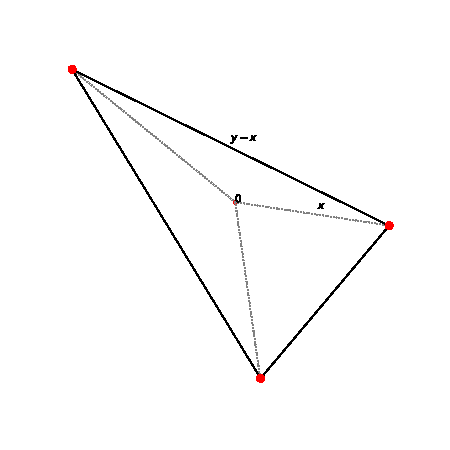
\includegraphics[width=\linewidth]{art/edgeconv-features.pdf}
        \end{column}
    \end{columns}
\end{frame}

\note[itemize]{
    \item Finally, the third theme in geometric methods is deep learning on
        graphs and other irregular data.
    \item A wide class of graph-convolutional models can be described in the language
        of message passing.
    \item For each node \( x \) in the graph, a message-passing model
        constructs feature vectors for all of its outgoing edges and aggregates
        them to produce a single output point.
    \item One example is the EdgeConv model, in which the message is
        formed by concatenation of the source vertex \( x \)
        and relative directions \( y - x \) towards the target vertices.
    \item Preceded with the dynamic nearest-neighbours graph construction,
        this model is used with pointclouds as well.
}

\begin{frame}{Experiments and results}
    \framesubtitle{\texttt{H-Conv 0.2}: ``Relative Directions''}

    \begin{columns}
        \begin{column}{.45\linewidth}
            \texttt{H-Conv 0.1}:

            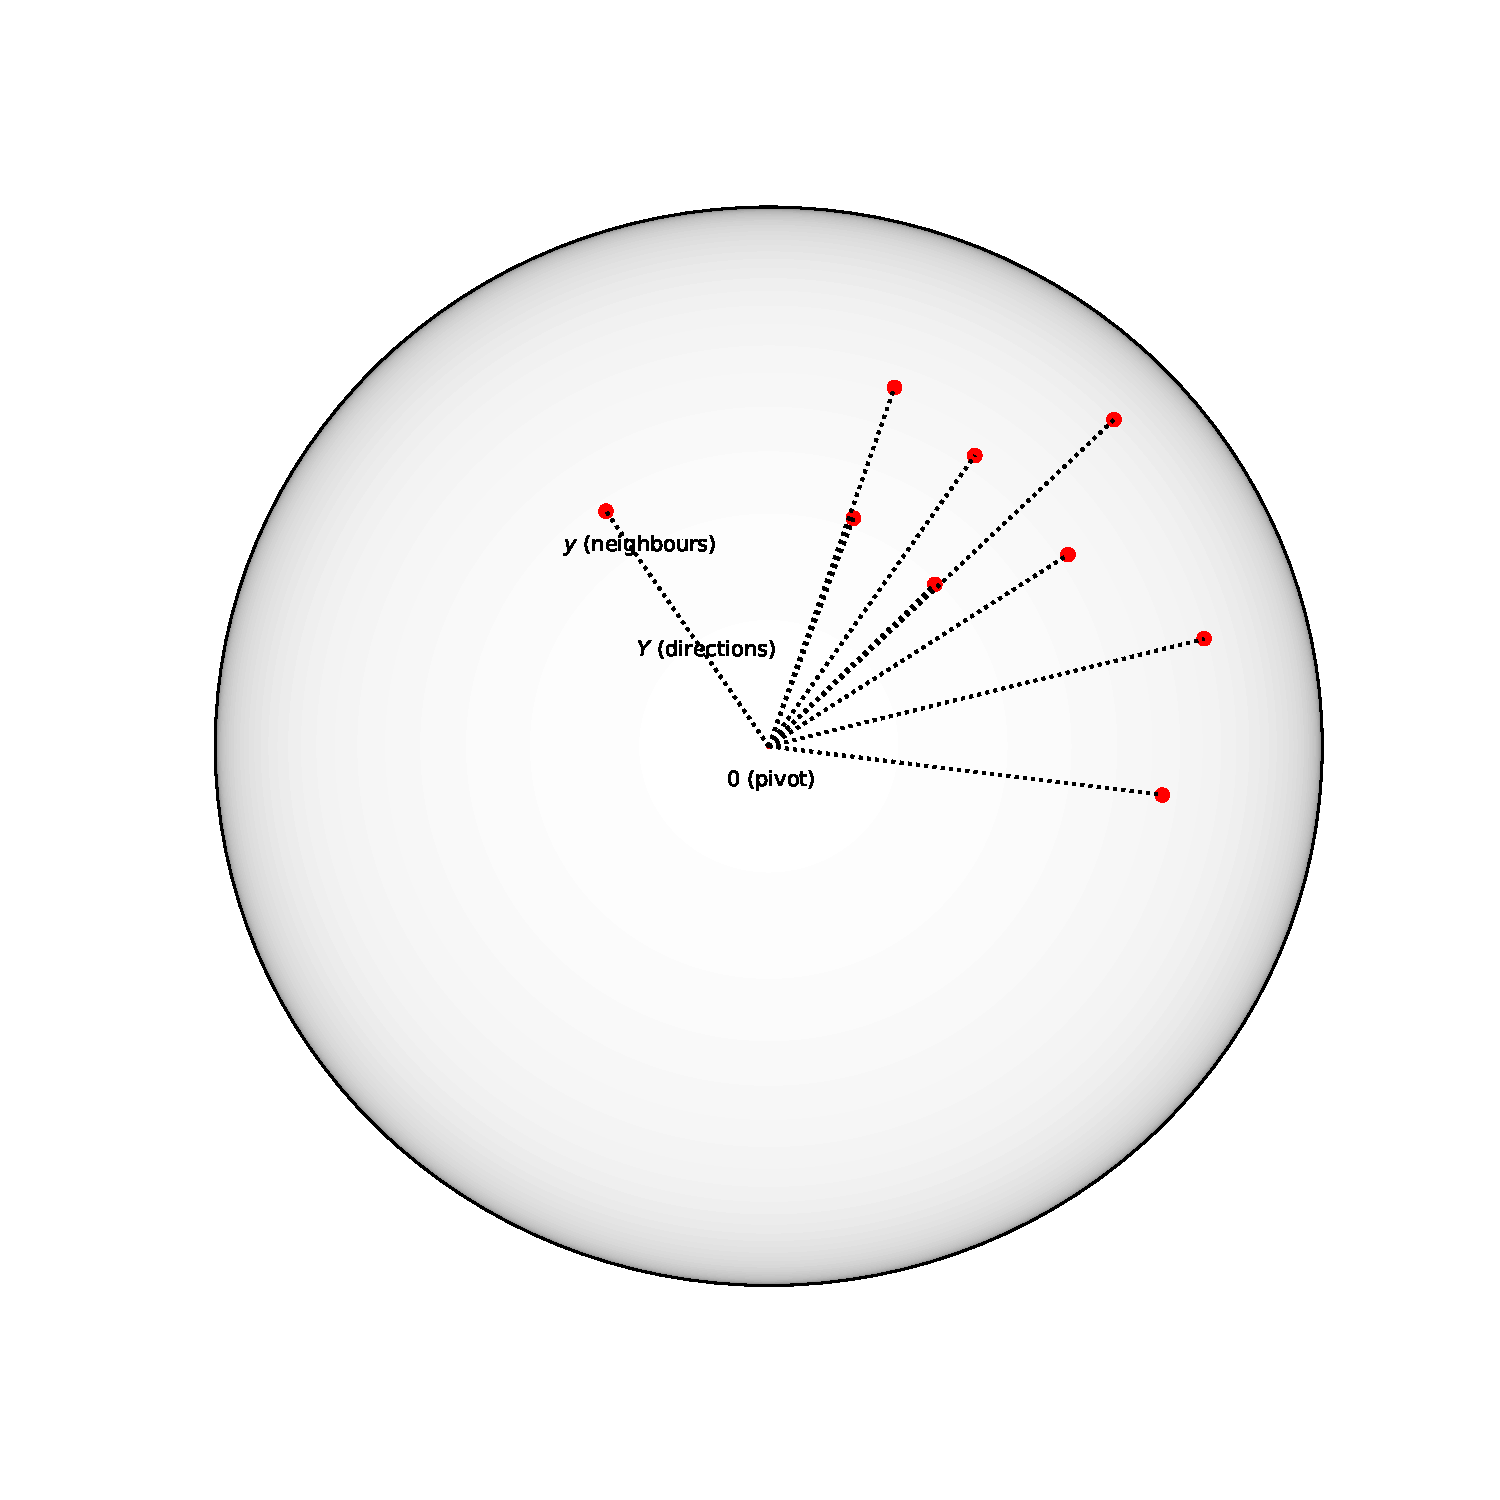
\includegraphics[width=.85\linewidth]{art/absolute-locations.pdf}
            \[ x' = \exp_0\left(
                \operatorname{Conv2D}\left(
                    \log_0 Y
                    \right)\right) \]
        \end{column}
        \begin{column}{.45\linewidth}
            \texttt{H-Conv 0.2}:

            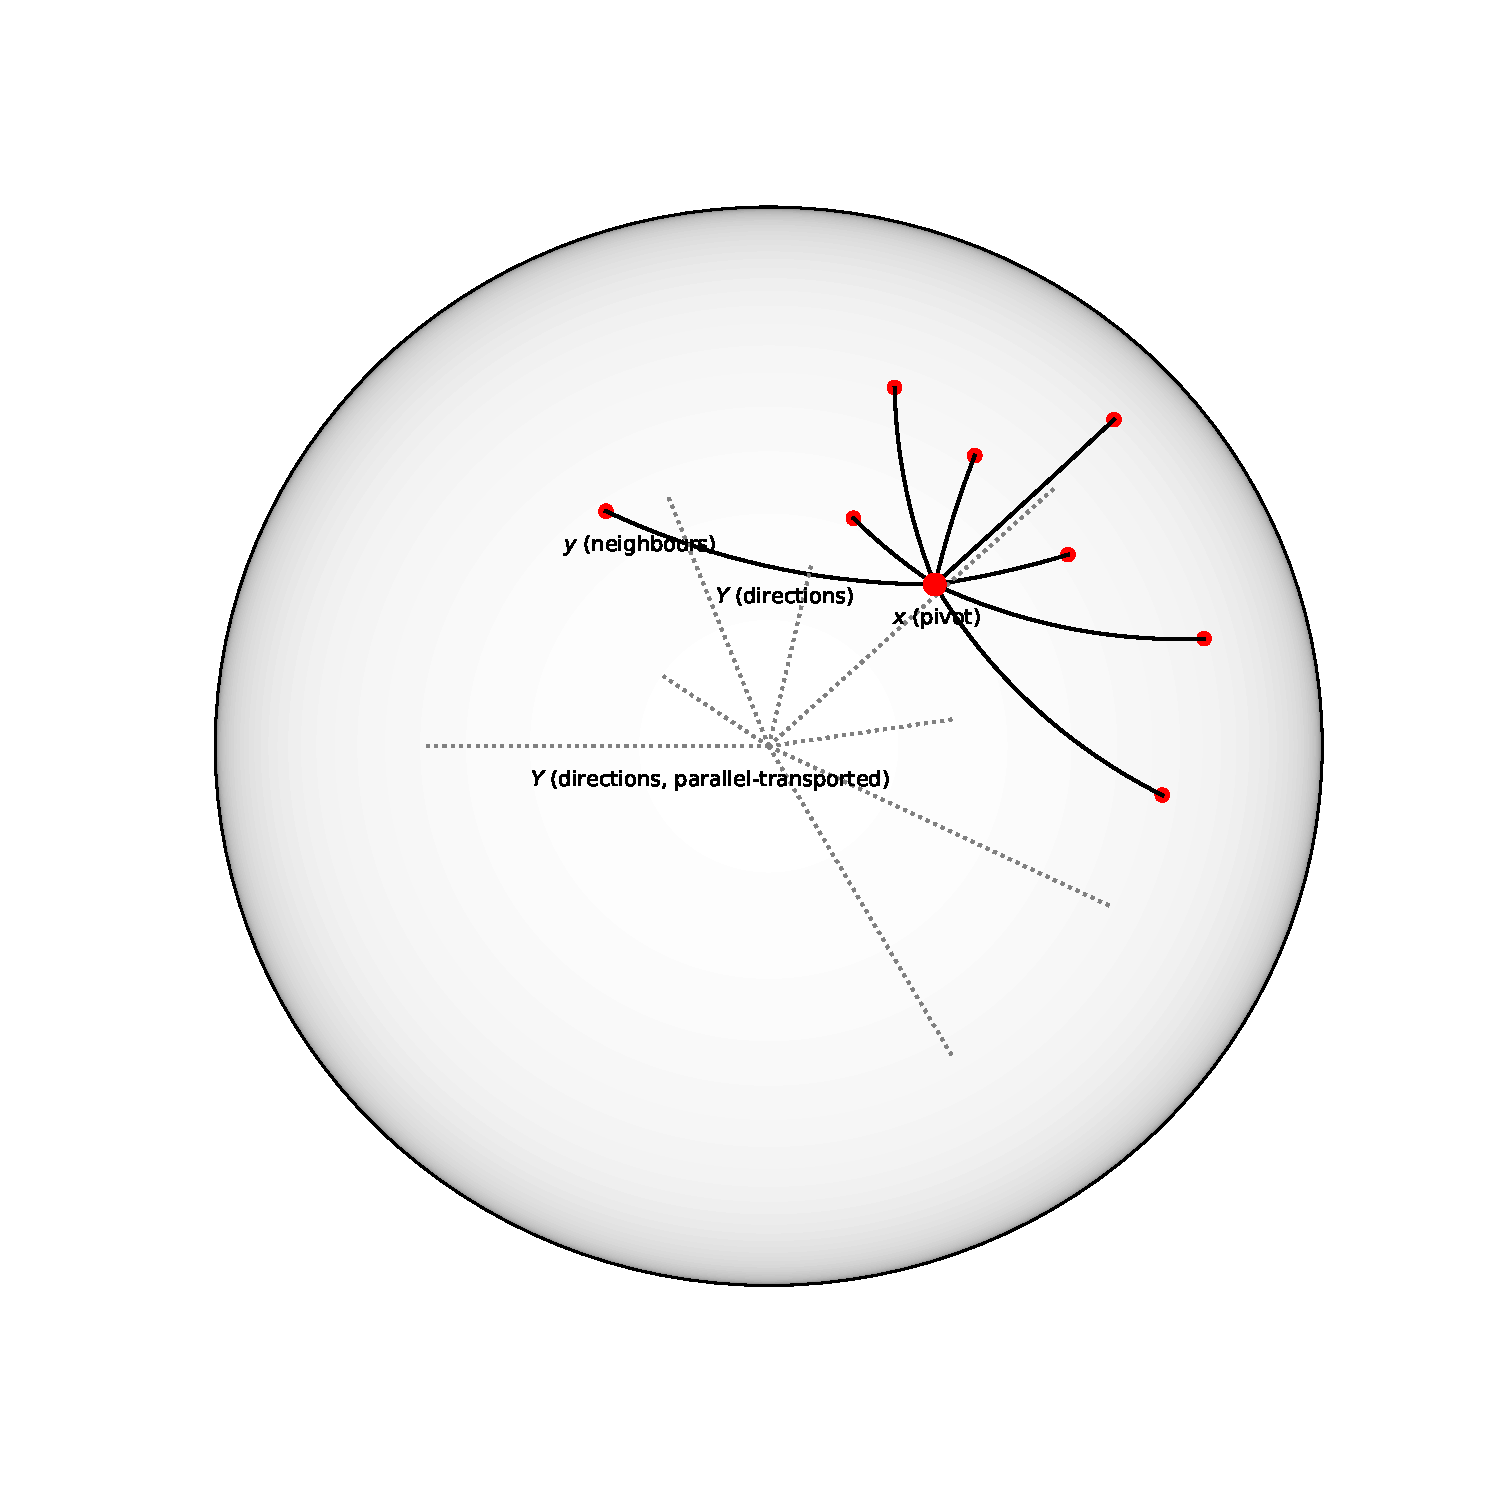
\includegraphics[width=.85\linewidth]{art/relative-locations.pdf}
            \[ x' = \exp_x\left(
                \operatorname{Conv2D}\left(
                    \log_x Y\right)\right) \]
        \end{column}
    \end{columns}
\end{frame}

\note[itemize]{
    \item Here we finish the discussion of the background and turn to
        contributions of the thesis.
    \item Consider in more detail the convolutional model we introduced
        for image classification.
    \item Each point in the sliding window can be represented by a shortest
        path from a fixed origin, denoted \( \log_0 Y \).
    \item Shortest paths emanating from a point, form a vector space.
    \item To these vectors we can apply the usual convolution,
        resulting in a new shortest path, and in turn a new point,
        denoted by \( \exp \).
    }
\note[itemize]{
    \item This operation doesn't commute with any of the isometries
        of the hyperbolic space.
    \item Our first step to fix this situation is to represent points by curves
        emanating from one the points in the window, as opposed to a fixed
        origin.
}

\begin{frame}{Experiments and results}
    \framesubtitle{\texttt{H-EdgeConv}}

    \begin{columns}
        \begin{column}{.4\linewidth}\centering
                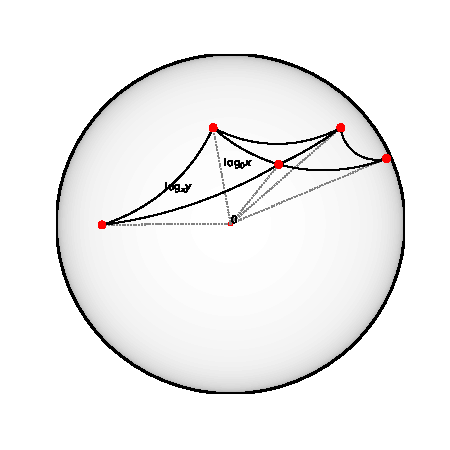
\includegraphics[width=.85\linewidth]{art/hedgeconv-features.pdf}
                \[\exp_o \operatorname{Conv2D}([\log_0x, \log_xy])\]
        \end{column}
        \begin{column}{.6\linewidth}
            \begin{table}[h!]
                \centering
                \begin{tabular}{|c c c c|} 
                    \hline
                    Model & params &
                    pts & acc
                    \\ [0.5ex] 
                    \hline\hline
                    \texttt{EdgeConv} & \( 1 \)M & \(1024\) & \(.90\)  \\ 
                    {\small 3DShapeNets} & \( 5 \)M & \(1024\) & \(.77\)  \\ 
                    \texttt{H-EdgeConv} & \( 85 \)K & 768 &  \( .71 \) \\ [1ex] 
                    \hline
                \end{tabular}
                \caption{Classification of Modelnet40 pointclouds}
            \end{table}

            \texttt{H-EdgeConv} is a combination of \texttt{H-Conv 0.\{1,2\}}
            plus \(k\)-NN graph instead of a regular grid of an image
        \end{column}
    \end{columns}
\end{frame}

\note[itemize]{
    \item Second step was generalization of EdgeConv layer to points on a
        manifold.
    \item The generalization is straightforward replacment of \( y - x \)
        by the geodesic connecting \( x \) to \( y \).
    \item This model generalizes the previously introduced ``hyperbolic array
        convolutions'' from implicit regular grids to graphs.
    \item This model has been evaluated on classification of pointclouds
        from the Modelnet40 dataset.
    \item With orders of magnitude fewer parameters, our model gives accuracy
        comparable to the baselines.
    \item Scaling to larger networks is, however, an open problem.
}

\begin{frame}{Experiments and results}
    \framesubtitle{Publications}
    
    \begin{itemize}
        \item (ELLIS) geoopt,~\citet{geoopt}
        \item (under review) denoising,~\citet{denoisingAkhmedkhan}
    \end{itemize}
\end{frame}

\note[itemize]{
    \item The artifacts of the work on this thesis include the Riemannanian
        optimization package Geoopt and other co-authored works...
    \item ...but, I believe, more is coming when I finally obtain positive
        results.
}

\begin{frame}{Discussion}
    \begin{itemize}
        \item Points in the window (neighbourhood) -- ``a discrete signal on~\( \mathbb{D} \)'':
            \( \frac1n \sum_{i=1}^n \delta_{x_i} \)
        \item Other functional bases than \( \delta_x \)?~\cite{stollharmonic}
        \item \( \log_xy \) is only invariant wrt M\"obius addition
        \item \(x\mapsto \int_{\mathcal{A}} f(\phi~0) h(\phi^{-1}x) \operatorname{d}\phi \),
            more in~\cite{stollharmonic}
        \item Broader class of problems, e.g. correspondence detection\&description
    \end{itemize}
\end{frame}

\note[itemize]{
    \item There are several ways in which I intend to improve this work.
    \item Cohen et al set the stage for convolutional networks as transforming
        ``signals on some symmetric space''.
    \item We can interpret the points in the window in our model
        as a discrete signal in the hyperbolic space.
    \item It could be useful to consider a subspace spanned by different basis
        functions, for example the spherical harmonics.
    \item In our \texttt{H-Conv} we fixed the ``translational'' component
        but not, for example, rotational one
    \item There are more isometries of Hyperbolic space and we could try to compute
        an explicit integral over all of them as in Cohen
    \item Finally, we used classification as a playground, but there are many more
        Vision tasks we're interested in.
}

\begin{frame}{Acknowledgements}
    Max Kochurov, Dmitry Ulyanov, Thibaut Le Gouic, Rasoul Karimov, and many,
    many others.
\end{frame}

\note{
    There's a huge list of people without whom this thesis wouldn't exist,
    but in time given, I should restrict myself to mentioning:
    my colleagues, Max Kochurov and Rasoul Karimov;
    I thank Dmitry Ulyanov and Thibaut Le Gouic who had guided and supervised
    me at different times during my Master's.
}

\begin{frame}{References}
    \printbibliography
\end{frame}

\end{document}

